\documentclass[12pt]{article}
\usepackage[T1]{fontenc}
\usepackage[a4paper, total={7in, 10in}]{geometry}
\usepackage{graphicx}
\usepackage[export]{adjustbox}
\usepackage[font=normalsize,labelfont=bf]{caption}
\usepackage{caption}
\usepackage{subcaption}
\usepackage{float}
\usepackage{titling}
\usepackage{fancyhdr}
\usepackage{lipsum}

\title{Modernizacja Laboratorium Drgań}
\author{Mateusz Klisiewicz}
\newcommand{\mytitle}{Modernizacja Laboratorium Drgań Mechanicznych}
\newcommand{\mysubtitle}{Plan Modelowy}
\fancyfoot{}
\fancyhead[L]{\mytitle}
\fancyhead[R]{\mysubtitle}

\fancyfoot[C]{\thepage}

\date{\today}



\renewcommand\maketitlehooka{\null\mbox{}\vfill}
\renewcommand\maketitlehookd{\vfill\null}
\renewcommand{\figurename}{Rysunek}
\graphicspath{{./tex_resources/}}
\title{\mytitle \\
  \large \mysubtitle}


\begin{document}
\maketitle
\newpage
\section*{Wstęp}
Poniższy plan ma na celu przedstawić rozwiązania dążące do ustandaryzowania, usprawnienia i ogólnej modernizacji eksperymentów wykonywanych w ramach Laboratorium Drgań Mechanicznych. W obecnej formule, istotna część zajęć często polega na rozwiązywaniu problemów technicznych i manualnej obróbce danych, przez co istota przeprowadzanego doświadczenia, a więc modelowanie i badanie zjawisk fizycznych, jest marginalizowana i niejednokrotnie pozostawiona bez wyjaśnień. \\Proponuje się zupełną zmianę podejścia do metody prowadzenia zajęć i przewartościowania wymagań stawianych studentom.
\section*{Laboratoryjna Aplikacja Komputerowa}
Proces modernizacji orientowałby się wokół aplikacji komputerowej, która w zamyśle oferowałaby zestaw nowoczesnych, atrakcyjnych wizualnie i intuicyjnych interfejsów, umożliwiających komunikację z układami elektronicznymi poszczególnych stanowisk pomiarowych.\\ W pierwszym etapie renowacji program obsługiwałby eksperymenty wykonywane na potrzeby Laboratorium Drgań Mechanicznych. Docelowo aplikacja miałaby się stać nieodłączną częścią wydziałowych przedmiotów laboratoryjnych i kluczowym elementem zajęć. 
\begin{figure}[h]
\centering
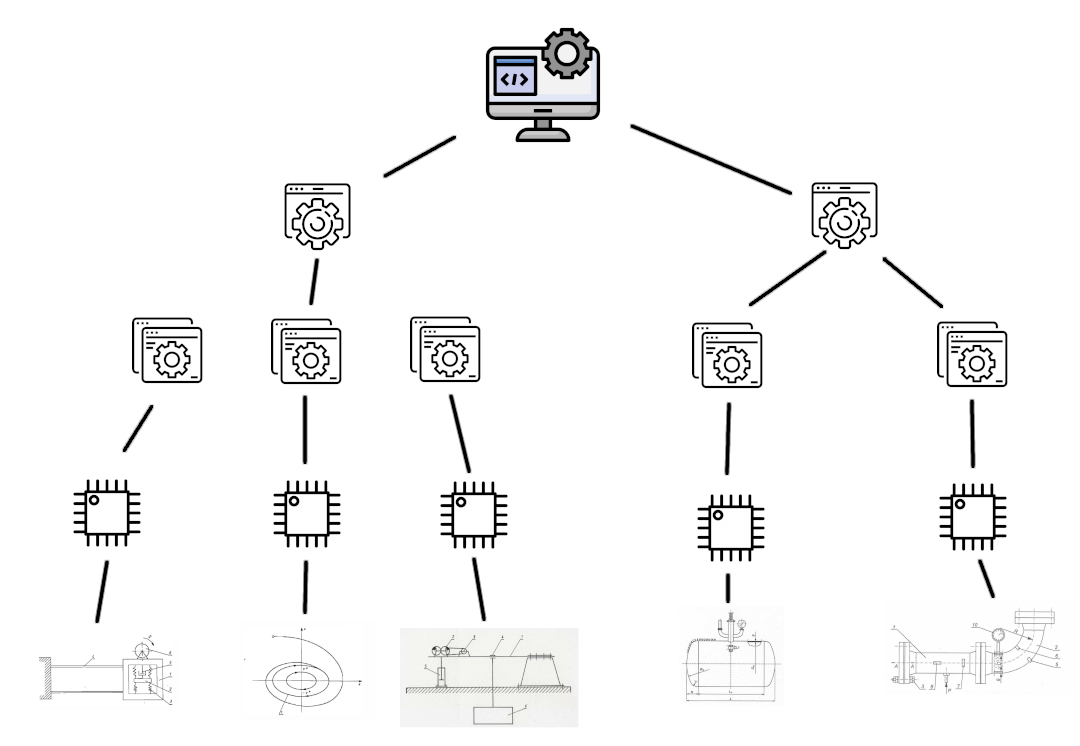
\includegraphics[width=14cm]{app_sch}
\caption{Schemat ideowy aplikacji laboratoryjnej}
\end{figure}
\newpage
\section*{Założenia}
Współcześnie, z dużą pewnością można założyć, że znacząca większość studentów posiada komputer przenośny
\end{document}